\subsection{Langkah Praktikum: Coin Exchange}

\subsubsection*{Flowchart}
\begin{figure}[H]
    \centering
    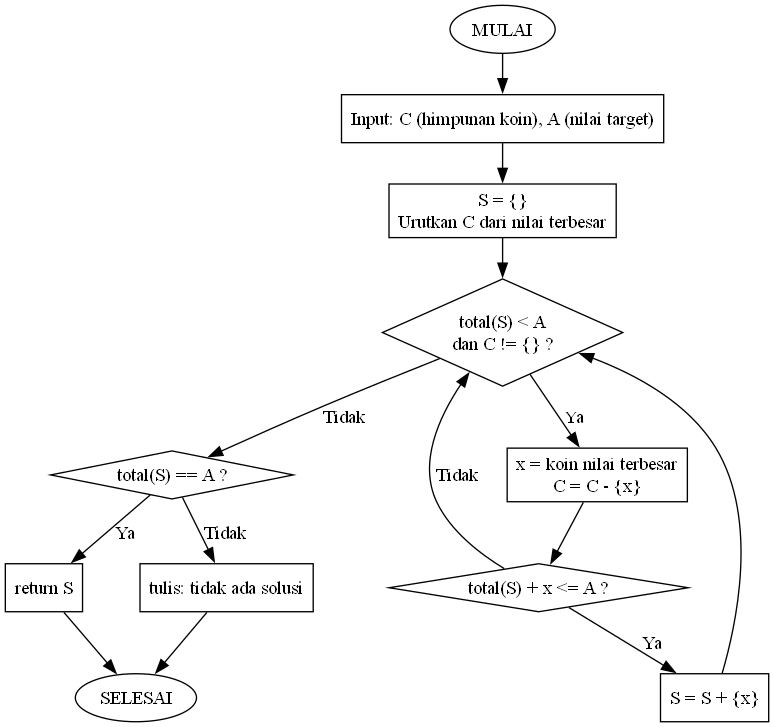
\includegraphics[width=0.55\textwidth]{figures/praktikum3/flowchart_coin_exchange.png}
    \caption{Flowchart Algoritma Coin Exchange}
\end{figure}

\subsubsection*{Source Code Python}
\begin{lstlisting}[basicstyle=\ttfamily\scriptsize, frame=single, backgroundcolor=\color{white}, numbers=none, keywordstyle=\color{black}, commentstyle=\color{black}, stringstyle=\color{black}, breaklines=true]
def coin_exchange(coins, amount):
    # urutkan koin dari nilai terbesar ke terkecil (strategi greedy)
    coins_sorted = sorted(coins, reverse=True)
    result = []
    remaining = amount

    for coin in coins_sorted:
        # ambil koin sebanyak mungkin selama tidak melebihi sisa
        while remaining >= coin:
            result.append(coin)
            remaining -= coin

    if remaining == 0:
        return result
    else:
        return None  # tidak ada solusi
\end{lstlisting}

\subsubsection*{Analisis Output}
Program diuji dengan koin standar [1000, 500, 200, 100, 50, 25, 10, 5, 1] dan nilai target 2750:

\begin{table}[H]
    \centering
    \caption{Proses Penukaran Koin dengan Pendekatan Greedy}
    \begin{tabular}{lll}
    \toprule
    \textbf{Langkah} & \textbf{Koin Dipilih} & \textbf{Sisa Nilai} \\ \midrule
    1 & 1000 & 1750 \\
    2 & 1000 & 750 \\
    3 & 500 & 250 \\
    4 & 200 & 50 \\
    5 & 50 & 0 \\ \bottomrule
    \end{tabular}
\end{table}

Hasil: koin yang digunakan = [1000, 1000, 500, 200, 50], total 5 koin. Algoritma greedy berhasil menemukan solusi minimal karena sistem koin Rupiah bersifat kanonik, artinya pilihan koin terbesar di setiap langkah selalu mengarah ke solusi dengan jumlah koin minimum.

\subsection{Post Test}

\subsubsection*{Source Code Python}
\begin{lstlisting}[basicstyle=\ttfamily\scriptsize, frame=single, backgroundcolor=\color{white}, numbers=none, keywordstyle=\color{black}, commentstyle=\color{black}, stringstyle=\color{black}, breaklines=true]
def analisis_kasus(coins, amount, label=""):
    print(f"\n{'='*50}")
    if label:
        print(f" {label}")
    print(f"{'='*50}")
    print(f"Nilai ditukar : {amount}")
    print(f"Koin tersedia : {sorted(coins, reverse=True)}")

    hasil = coin_exchange(coins, amount)

    if hasil:
        rekap = Counter(hasil)
        print(f"Solusi        : {dict(rekap)}")
        print(f"Jumlah koin   : {len(hasil)}")
    else:
        print("Tidak ada solusi (greedy gagal).")

    return hasil

def hitung_kompleksitas(coins, amount):
    # hitung iterasi aktual untuk analisis kompleksitas
    coins_sorted = sorted(coins, reverse=True)
    n = len(coins_sorted)
    iterasi = 0
    remaining = amount

    for coin in coins_sorted:
        while remaining >= coin:
            remaining -= coin
            iterasi += 1

    print(f"\nAnalisis Kompleksitas (amount={amount}, n={n} jenis koin):")
    print(f"Jumlah iterasi while : {iterasi}")
    print(f"Jumlah iterasi for   : {n}")
    print(f"T(n) = O(n + amount/koin_terkecil) -> praktis O(n) untuk denominasi wajar")

if __name__ == "__main__":
    koin_std = [1000, 500, 200, 100, 50, 25, 10, 5, 1]

    # kasus 1: solusi optimal
    analisis_kasus(koin_std, 2750, "Kasus 1: Solusi Normal")

    # kasus 2: jumlah besar
    analisis_kasus(koin_std, 9875, "Kasus 2: Jumlah Besar")

    # kasus 3: greedy tidak optimal (denominasi tidak kanonik)
    koin_non_kanonik = [10, 6, 1]
    analisis_kasus(koin_non_kanonik, 12, "Kasus 3: Greedy Tidak Optimal (koin [10,6,1], target 12)")
    print("  Solusi greedy: 10+1+1 = 3 koin")
    print("  Solusi optimal: 6+6   = 2 koin")

    # analisis kompleksitas
    hitung_kompleksitas(koin_std, 2750)
\end{lstlisting}

\textbf{Jawaban 1: Implementasi, output, dan analisis kasus}\\
Program diuji pada tiga kasus:
\begin{itemize}
    \item \textbf{Kasus 1 (nilai 2750, koin kanonik):} Solusi = \{1000:2, 500:1, 200:1, 50:1\}, total 5 koin. Greedy optimal.
    \item \textbf{Kasus 2 (nilai 9875, koin kanonik):} Solusi = \{1000:9, 500:1, 200:1, 100:1, 50:1, 25:1\}, total 14 koin. Greedy optimal.
    \item \textbf{Kasus 3 (nilai 12, koin [10,6,1] non-kanonik):} Solusi greedy = \{10:1, 1:2\} = 3 koin. Solusi optimal = \{6:2\} = 2 koin. Greedy tidak optimal karena sistem koin tidak kanonik.
\end{itemize}

Kasus 3 membuktikan bahwa algoritma Greedy tidak menjamin solusi optimal secara universal. Untuk sistem koin non-kanonik, diperlukan pendekatan Dynamic Programming.

\textbf{Jawaban 2: Kompleksitas waktu}\\
Analisis kompleksitas dilakukan berdasarkan dua komponen utama:
\begin{itemize}
    \item \textbf{Loop for iterasi jenis koin:} dilakukan sebanyak n kali (n = jumlah jenis koin). Kompleksitas O(n).
    \item \textbf{Loop while pengambilan koin:} untuk setiap jenis koin, jumlah pengambilan bergantung pada nilai koin dan sisa amount. Dalam kasus terburuk total iterasi while = floor(A / koin\_terkecil).
\end{itemize}

Sehingga total kompleksitas:
\[ T(n) = O(n + A / d\_min) \]

dengan n = jumlah jenis koin dan d\_min = nilai koin terkecil. Untuk sistem mata uang praktis (d\_min = 1), kasus terburuk adalah T(n) = O(A). Namun secara praktis karena koin terbesar mendominasi pengambilan, jumlah iterasi while jauh lebih kecil dari A sehingga kompleksitas efektif mendekati O(n).

\begin{table}[H]
    \centering
    \caption{Kompleksitas Waktu Algoritma Coin Exchange}
    \begin{tabular}{ll}
    \toprule
    \textbf{Komponen} & \textbf{Kompleksitas} \\ \midrule
    Pengurutan koin (sorting) & O(n log n) \\
    Iterasi jenis koin (for) & O(n) \\
    Pengambilan koin per jenis (while) & O(A / d\_min) worst case \\
    \midrule
    Total keseluruhan & O(n log n + A / d\_min) \\ \bottomrule
    \end{tabular}
\end{table}